\section{Frontend}

Das Fronted der TeamDocument Applikation ist als React SPA entwickelt.
Einmal angemeldet kann ein Benutzer an der kollaborativen Bearbeitung des Dokumentes teilnehmen.

Folgende Interaktionen sind möglich:

\begin{itemize}
    \item Ändern des eigenen Namens
    \item Hinzufügen eines neuen Paragrafen
    \item Bearbeitung bestehender Paragrafen
    \item Sperren des Paragrafen an dem gerade gearbeitet wird (implizit)
    \item Verschieben von Paragrafen innerhalb des Dokuments
    \item Löschen eines bestehenden Paragrafen
    \item Wiederherstellen des zuletzt gelöschten Paragrafen (Hidden Feature)
\end{itemize}

Des Weiteren werden folgende Informationen auf dem UI dargestellt:

\begin{itemize}
    \item Name des ursprünglichen Authors eines Paragrafen
    \item Name des Authors welcher aktiv einen Paragrafen bearbeitet.
    \item Highlight des eigenen aktuellen Paragrafen
    \item Liste mit allen Dokumentupdates in chronologischer Reihenfolge
    \item Avatare aller aktiven Benutzer
\end{itemize}

\begin{figure}[H]
    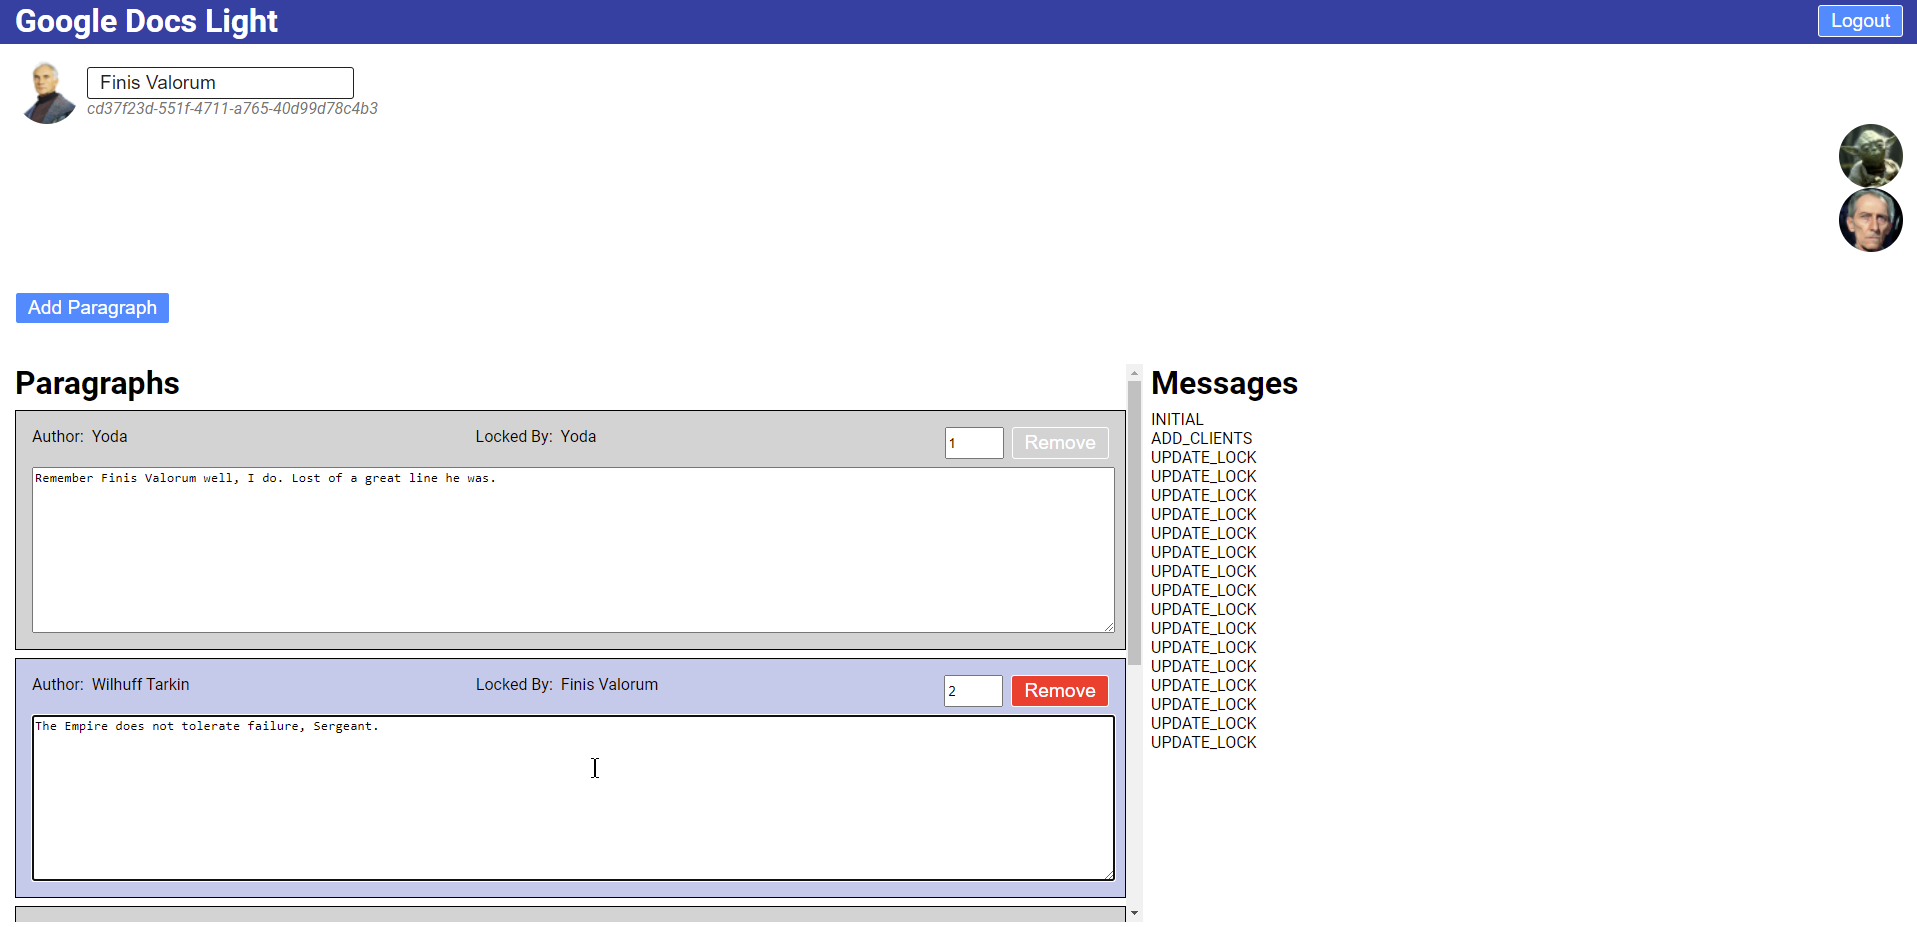
\includegraphics[width=\textwidth,keepaspectratio]{UI-blank}
    \caption{Team Document User Interface}
    \label{fig:Team Document User Interface}
\end{figure}


\subsection{Aufbau}

Die UI-Elemente sind als React-Komponenten umgesetzt und hierarchisch gegliedert.
Einzelne Komponenten nutzen zusätzliche Funktionalität, die in kleine Service Module ausgelagert ist.

Die Anbindung ans Backend ist mit zwei unidirektionalen Kanälen realisiert.

Der State der gesamten Applikation wird vom Redux Store bewirtschaftet.

\begin{figure}[H]
    \centering
    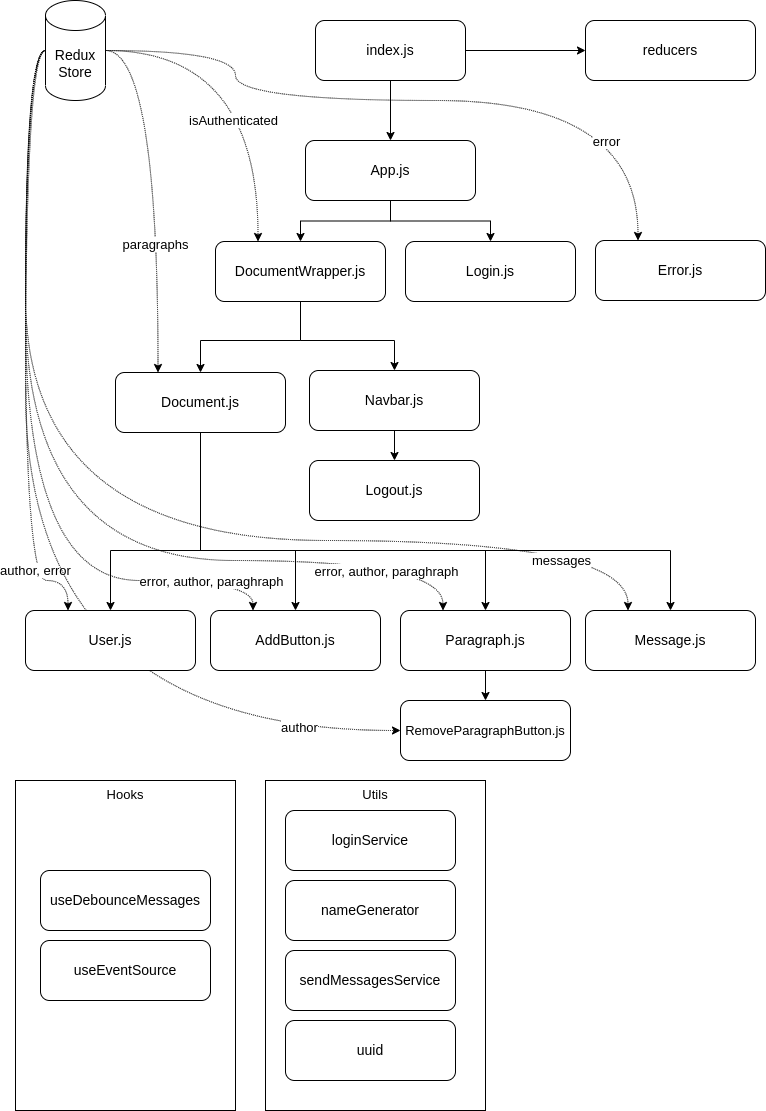
\includegraphics[width=\textwidth,keepaspectratio]{fe_structure}
    \caption{Komponenten Struktur}
    \label{fig: Fe_Structure}
\end{figure}

\subsubsection*{index.js}
Das Index File ist der Eintrittspunkt für den Browser.
Beim Laden der Applikation wird der Redux Store erstellt und initialisiert.
Ebenfalls wird im Local Storage des Browsers geprüft, ob bereits ein User registriert ist.
Ist dies nicht der Fall, so wird ein zufälliger Benutzer generiert.

\subsubsection*{App.js}
Die App Komponente ist das äusserste Element, welches alle anderen Elemente hält.
Wir verwenden einen BrowserRouter um zwischen dem eigentlichen Dokument und der Login-Seite zu navigieren.

\subsubsection*{DocumentWrapper.js}
Wrapper um das Dokument zu schützen.
Solange sich ein User noch nicht ordentlich am Backend authentifiziert hat, leitet diese Komponente den Benutzer stetig auf die Login-Page weiter.

\subsubsection*{Login.js}
Login Formular, welches den Login Service verwendet.
Das Formular übersetzt die eingegebenen Credentials in einen Basic Auth Header und sendet damit einen GET Request ans Backend.
Bei erfolgreicher Authentifizierung wird das User Principal im Local Storage abgelegt.

\subsubsection*{Error.js}
Generische Fehlermeldung, welche als modales PopUp angezeigt wir, im Falle eines fehlgeschlagenen Requests.

\subsubsection*{Document.js}
Document ist der Parent des eigentlichen Dokuments.
Hauptsächlich ist sie dafür verantwortlich alle Paragrafen sortiert darzustellen.

\subsubsection*{Navbar.js}

\begin{figure}[H]
    \centering
    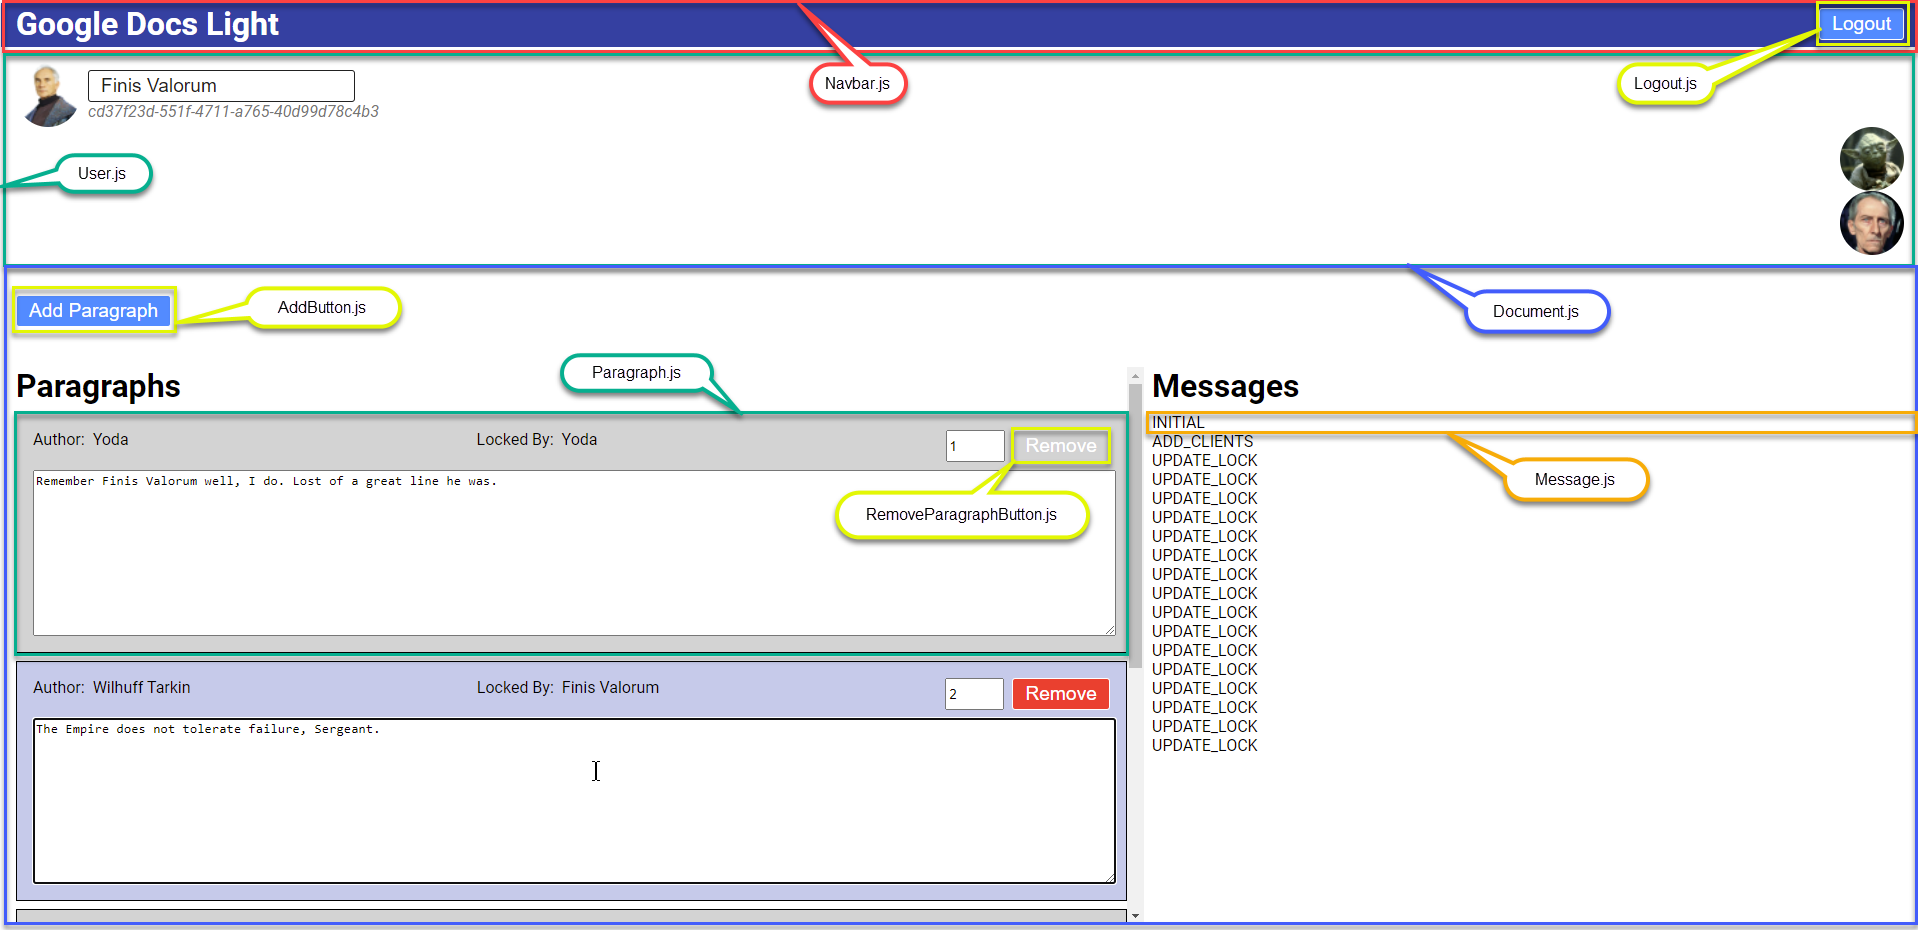
\includegraphics[width=\textwidth,keepaspectratio]{UI-components}
    \caption{UI-Components}
    \label{fig: UI-Components}
\end{figure}

\subsection{Ablaufdiagram}

\begin{figure}[H]
    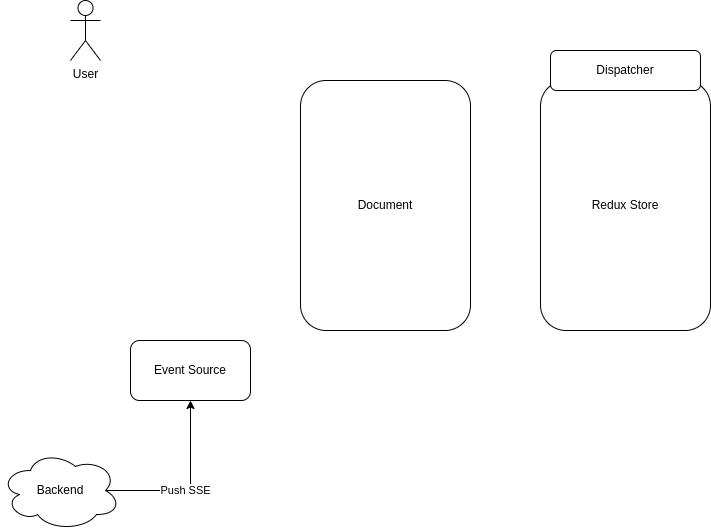
\includegraphics[width=\textwidth,keepaspectratio]{fe_dataflow}
    \caption{Datenfluss}
    \label{fig:}
\end{figure}


\subsection{State- und Konfliktmanagment}
%Redux State Verwaltung

\subsection{Fehler Behandlung}
